\documentclass[11pt,twoside,a4paper,openright]{report}

\usepackage[utf8]{inputenc}
\usepackage[english]{babel}
\usepackage{lmodern}
\usepackage[T1]{fontenc}
\usepackage[table]{xcolor}
\definecolor{aaublue}{RGB}{33,26,82}
\usepackage{graphicx}
\usepackage{tabularx}
\usepackage{caption}
\captionsetup{%
  font=footnotesize,
  labelfont=bf 
  }
\usepackage{array,booktabs}
\usepackage{wrapfig}
\usepackage{adjustbox}
\usepackage{framed}
\usepackage{amsmath}
\usepackage{amssymb}
\usepackage[framed,amsmath,thmmarks]{ntheorem}
\usepackage{dblfloatfix}
\usepackage{adjustbox}
\usepackage{layouts}
\usepackage{lipsum}
\usepackage{pdfpages}
\usepackage{verbatim}
\usepackage{rotating}


\usepackage[
  left=0.5in,
  right=0.5in,
  bottom=1mm,
  top= 1in,
  ]{geometry}
\usepackage{titlesec}
\titleformat*{\section}{\normalfont\Large\bfseries
    }
\titleformat*{\subsection}{\normalfont\large\bfseries
    }
\titleformat*{\subsubsection}{\normalfont\normalsize\bfseries
    }
%\titleformat*{\paragraph}{\normalfont\normalsize\bfseries}}
%\titleformat*{\subparagraph}{\normalfont\normalsize\bfseries}}


% configure section titles
\usepackage{titlesec}
\titleformat{\section}{\Large\bfseries}{\thesection}{1em}{}
\titleformat{\subsection}{\large\bfseries}{\thesubsection}{1em}{}

\begin{document}
% custom commands
\newcommand{\windef}[1]{\subsection*{\underline{DEF:} \normalsize{#1}}} % definition
\newcommand{\winex}[1]{\subsection*{\underline{EX:} \normalsize{#1}}} % example
\newcommand{\winsec}[2]{\section*{\underline{\textbf{#1}}{#2}}} % section
\newcommand{\winres}[1]{\begin{math}\Rightarrow\left\{\begin{matrix}#1\end{matrix}\right.\end{math}\hspace{0.2cm}} % result
\newcommand{\winsys}[1]{\begin{math}\left\{\begin{matrix}#1\end{matrix}\right.\end{math}} % system
\newcommand{\winero}[1]{\begin{math}\xrightarrow{#1}\end{math}} % row operation
\newcommand{\winmat}[1]{\begin{math}\begin{bmatrix}#1\end{bmatrix}\end{math}} % matrix
\newcommand{\winsub}[1]{\subsection*{\hspace{0.2cm}\textit{ #1}}} % dot
\newcommand{\step}[1]{\begin{math}\xrightarrow{\text{#1}}\end{math}} % step in a process
\newcommand{\winrtwo}{\begin{math}\text{R}^\text{2}\end{math}}
\newcommand{\winrthree}{\begin{math}\text{R}^\text{3}\end{math}}
\newcommand{\wineq}[1]{\begin{equation}\notag#1\end{equation}}
\newcommand{\winans}[1]{\begin{equation}\underline{\underline{\notag\boldsymbol{#1}}}\Leftarrow\end{equation}}
\newcommand{\horrule}[1]{\rule{\linewidth}{#1}} % Create horizontal rule command with 1 argument of height



\begin{comment}
\begin{titlepage}

\vfil
	\centering
	{\huge\bfseries PSAS Liquid Propellant Rocket Engine
Electric Feed System\par}
	\vspace{0.5cm}
	{\scshape\Large Conceptual Design Progress Report\par}% Insert Document title here

\vspace{5cm}

	{\Large\itshape 	{Jorden Roland, 
John Froehlich,\\
James Luce, 
Mimi Shang,\\
John Talik, 
Rawand Rasheed\par}}

\vspace{3cm}
Faculty advisor:\par
    \textsc{Ra\'{u}l Bayo\'{a}n Cal}\par
	Supervised by:\par
    \textsc{Erin Schmidt}\\
	and\\
	\textsc{Andrew Greenberg}

	\vspace{3cm}
	
%textwidth in cm: \printinunitsof{cm}\prntlen{\textwidth}

\begin{table*}[!t]

  \begin{tabular}{  p{2cm}  m{13.20337cm}  p{2cm}  }
  
\\ \hline

\begin{minipage}{.3\textwidth}
 \begin{flushleft}
      
\includegraphics[width=0.3\textwidth]{logo.png}
 \end{flushleft}
\end{minipage}

&

\begin{center}
	{Portland State Aerospace Society}\par
	{Fariborz Maseeh College of Engineering and Computer Science}\par
	{\large \today \par}
	\end{center}

&	

\begin{minipage}{.3\textwidth}
%\begin{flushright}
      
\includegraphics[width=0.3\textwidth]{psas_insignia.png}
%      \end{flushright}
    \end{minipage}\\ \hline
   
\end{tabular}
\end{table*}


\end{titlepage}
\newgeometry{top=1in,bottom=1in,right=1in,left=1in}
\newpage
\thispagestyle{empty}


\winsec{Executive Summary: }{}
\vspace{12pt}
The Electric Feed System (EFS) team will design, build, and test an electric feed system prototype to serve as a technology development platform for the PSAS LV4 rocket using commercial off the shelf (COTS) parts and in-house manufacturing by June 16, 2017 and for less than \$15,800.\par
\vspace{12pt}
As of the time of this report, the EFS project is developing the first prototype, which will use water as its working fluid, and is transitioning from design to fabrication and testing. The project is currently ahead of the milestone schedule established by the project plan. \par
\vspace{12pt}
Efforts over the last two months have largely focused on pump sizing and impeller design. The critical decision has been made to transition from theory to validation through physical experiment, allowing us to proceed with the first prototype test. Along with pump theory and design, there have been ongoing parallel efforts to complete the other tasks required for the first prototype test, such as development of controls and data acquisition systems, sensor calibration, completion of CAD design, and identification and acquisition of critical components such as a motor, speed controller, and battery.\par
\vspace{12pt}
Our next milestone is the finalization of detailed design, encompassing impeller design, COTS parts selection, system simulation, and CAD modeling for the first prototype, planned for 3/26/17 but nearly complete as of 3/17/17. The associated milestone of finishing COTS part purchasing, due 4/2/17, is also largely complete and should be finished by 3/24/17.\par
\vspace{12pt}
The two critical following milestones are the assembly and testing of the first prototype, originally planned for 4/24/17 and 5/6/17, respectively. These two steps are now anticipated to be completed by 3/31/17 and 4/7/17, as much of the work required to execute this first test is either complete, underway, or well planned for. The major tasks preceding the first prototype test will be fabrication of the pump assembly, procurement of miscellaneous remaining COTS parts, and assembly of the test apparatus.\par
\vspace{12pt}
Looking forward to the final deliverable of a tested second prototype using liquid oxygen as a working fluid, our current status encourages us that we will be able to confront the challenges exposed by physical testing and the development of the final prototype.\par
\vspace{4cm}

\begin{flushright}
\begin{tabular}[t]{@{}p{3.5in}@{}}
  \\[-2ex]
  \strut \textit{Signature: }\underline{\hspace{2.75in}}\strut
  \end{tabular}\\
  {Ra\'{u}l Bayo\'{a}n Cal}\\
Faculty advisor
\end{flushright}

\newpage

%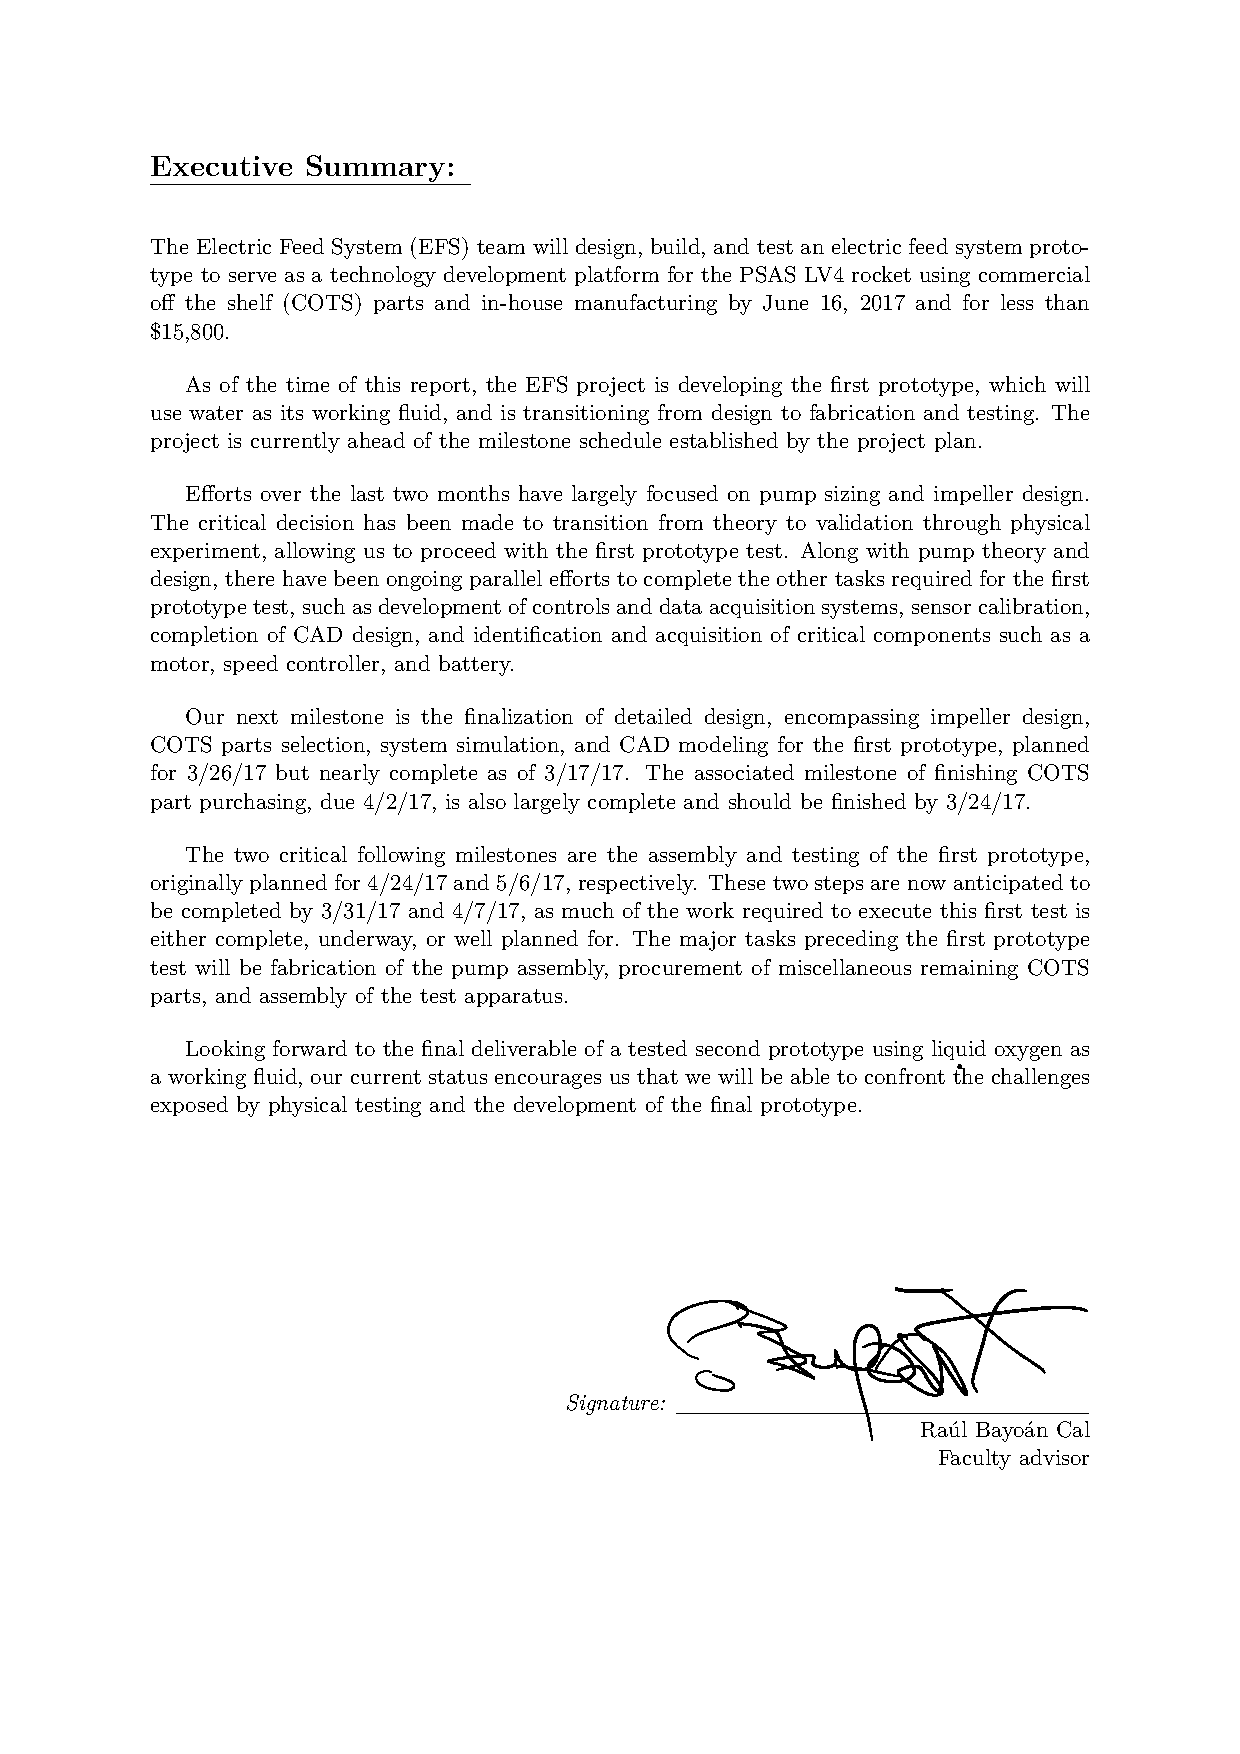
\includepdf{Summary_efs.pdf} <------This doesnt work for some reason.

\setcounter{page}{1}
\winsec{Conceptual Design Summary: }{}
\vspace{12pt}
The EFS project was provided to the team with most of the conceptual design decisions wrapped up in the engine/vehicle level requirements. The majority of complex decisions involving trade offs are occurring at an analytical level in the pump sizing process. For the EFS project, descisions regarding different propulsion types, such as solid motors, pressure fed liquid, or liquid turbopump engines have already been made. The EFS will use electric motor driven centrifugal pumps, powered by a lithium polymer batteries, using liquid oxygen (oxidizer) and isopropyl alcohol (fuel) as propellants, given a specific inlet pressure and producing a required flow rate and pressure head. Thus, for the EFS team, the highest level decisions were subsystem component level decisions, including choosing an impeller type and impeller housing design.\par
\vspace{12pt}
\winsub{Concept selection process: Impeller type}
\vspace{12pt}
For conventional pump design, the choice of impeller type would be a straightforward output of a pump sizing process and would not represent a major concept selection. The nature of the EFS project required a deeper investigation into impeller style, as the consequences this selection affects nearly all other subsystems. Typically, pump sizing calculations use a set of requirements to  produce a specific speed value, and impeller style is dictated by this value which dictates an impeller style. For example, a particular specific speed value might imply that a Francis vane impeller is more ideal than a normal radial vane impeller, see figure 1 below. The EFS project’s requirements specify an unusually high head and low flow rate, resulting in a specific speed requirement that falls outside of the ranges of common impeller types. \par
	
\begin{figure}[h]
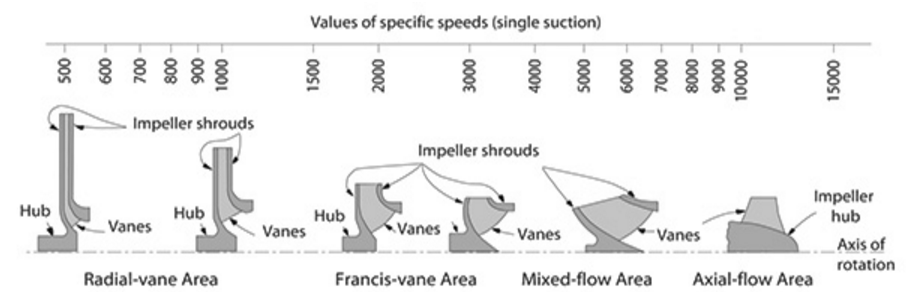
\includegraphics[width=\textwidth]{Ns_Impeller_type_bw.png}
\caption{Typical flow classification of pump impellers as per specific speed}
\end{figure}

\vspace{12pt}
This forced a radical departure from the typical options found in pump design documentation. Literature review outside of the normal canon of rocket pump design led to the exploration of a Barske design impeller: an unorthodox, straight vane radial impeller design suitable for low flow, high head, and low specific speed requirements.\par
\vspace{12pt}
The decision was made to proceed with designing the EFS system around a Barske impeller for two reasons: a Barske design is suitable for our pump’s specific speed range and it is easier to manufacture than more geometrically complex impellers. The downside of the Barske design is that it is not represented well in the common pump sizing documentation, and thus may require more experimental testing to characterize its performance. In our application, this is 
\newpage
\noindent
not necessarily a loss. As the performance requirements of the EFS largely fall outside of the regimes covered by common pump sizing documentation already, and thorough experimentation will be required for any approach. In other words, the unknown characteristics of Barske impellers is not a high risk, as the EFS' requirements put the impeller outside of common pump characteristics. Consequently, there was no perceived trade-off in the decision to proceed with a Barske impeller. A subsystem performance matrix interpreting this decision is included in the appendix.\par

\vspace{12pt}
%--------------------------------------------------------------------------------------------------------------------------%
%--------------------------------------------------begin screening matrix---------------------------------------------%
%--------------------------------------------------------------------------------------------------------------------------%
\begin{table*}[!h]
\caption{Screening matrix for impeller design choice}
\resizebox{\textwidth}{!}{%
\begin{tabular}{|c||c|c|c|}
\hline
                          &{Specific speed range} &{Manufacturability}&{Testing requirements}  \\ 
                          &{($<500$ is required)}&                           &                                    \\ \hline \hline
Common designs  &  & Very complex: investment casting & Designs are included \par  \\
(radial, Francis, mixed flow, axial) &500-8000 (too high)&or 5 axis milling of impeller and housing.&in pump sizing literature but requirements fall \\
&&&outside of common regimes.\\ \hline
Barske design &400-1000 (appropriate)&Very simple: impeller and housing&Not included in common literature and\\
&& can be made with 3 axis mill.&experimentation required to characterize.\\ \hline
\end{tabular}}

\end{table*}
%----------------------------------------------------------------------------------------------------------------------------%

\winsub{Concept selection process: Housing type}
\vspace{12pt}
Another major decision was to determine the housing type to be used for the initial prototype and water testing. A simple option for an impeller housing is a concentric design, which is the easiest to manufacture but may reduce efficiency and performance. Higher performance housing options might include an expanding volute or the addition of a cutwater to the concentric design. Figure 2 shows two potential options for housing design.\par

\vspace{12pt}
\begin{figure}[h]
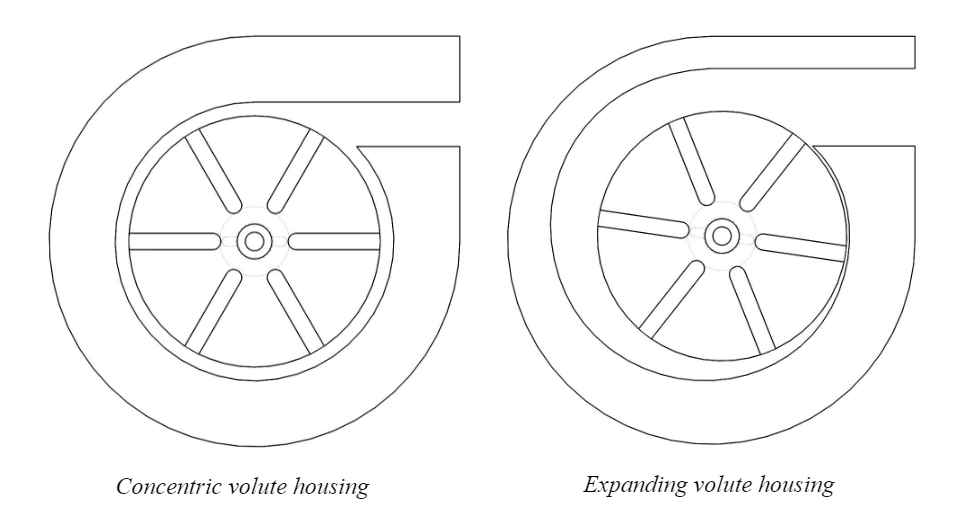
\includegraphics[width=\textwidth]{concentric_vs_volute.png}
\caption{Example of a concentric bowl design versus a non-concentric volute design}
\end{figure}

\newpage
The final product of the EFS project has high performance requirements that may require use of performance enhancing techniques, such as housing modifications like an expanding volute. The goal of the first prototype is to provide theory validation, not hit final performance targets, and thus has a unique set of requirements that differ from the second prototype's. For example, although the final prototype needs to achieve 350 psi at 11 gpm flow, the first prototype's true goal is to achieve performance in a range such that we can calibrate the assumptions in our theory to design the second prototype accordingly. \par
\vspace{12pt}
This difference in utility between the two prototype dictates the choice of housing type for the first prototype. While there is a benefit to seeing higher performance in the first prototype, there is the cost to having additional variables to consider when interpreting the first prototype test data. The first prototype test is intended to isolate the influence of factors represented in the pump sizing theory we are using for our fundamental design calculations. For example, impeller diameter, height, blade number, inlet size, and outlet size are critical dependent variables. Conveniently, many of these variables are connected, and a test regimen does not need to independently manipulate each variable. Introducing housing design as a dependent variable at this stage would dramatically complicates the testing required without providing clear validation of the theory used in the design.\par
\vspace{12pt}
%--------------------------------------------------------------------------------------------------------------------------%
%--------------------------------------------------begin screening matrix---------------------------------------------%
%--------------------------------------------------------------------------------------------------------------------------%
\begin{table*}[!h]
\caption{Screening matrix for housing type selection}
\resizebox{\textwidth}{!}{%
\begin{tabular}{|c||c|c|c|}
\hline
                                              &{Testing influence} &{Performance}&{Costs}  \\ \hline \hline
                                               &  May need to be designed and                            &&Significant design process.\\
Housing with expanding volute,  &  tested for second prototype anyway.                  & May bring us closer to target values. &Cannot be manufactured on lathe.\\
 cutwater, or other modifications & Introduces a unique variable to testing                &&\\
                                               & not represented in our pump sizing calculations.   &&\\ \hline
Concentric housing                    & Simplifies analysis of test data.                           & May cause low performance that&Simple to design.\\
                                               &   & complicates test data analysis.& Can be manufactured on lathe or 3 axis mill.\\ \hline
\end{tabular}}

\end{table*}
%----------------------------------------------------------------------------------------------------------------------------%
\winsub{Concept selection process: Impeller test design}
\vspace{12pt}
The most complex and consequential decision making in this project has involved the design of the impeller. A Python notebook is used to bring together equations incorporating performance requirements, fluid properties and geometric constraints to produce suggestions about impeller dimensions. Trade-offs here are complex. A change in RPM might benefit from a higher blade count which might introduce losses due to narrow fluid channels, while a lower blade count may induce pressure fluctuations, etc.\par
\vspace{12pt}
Given that our application is near the limit of pump sizing regimes, there is significant uncertainty in the design process. For the first prototype, the goal is to produce a set of possible impeller geometries that allow isolation of some of these significant unknowns. Performing experimental runs with combinations of impeller diameter, blade number, and blade tip height will allow a better understanding of pump theory, Barske design behavior, and the hydrodynamic regime that the EFS exists in (Figure 4). The variations of impeller and housing geometries are passed to parameterized CAD drawings designed for machinability (Figure 3). Additionally, the blade geometries are checked  for strength concerns using static finite element analysis.\par

\vspace{12pt}
\begin{figure}[!h]
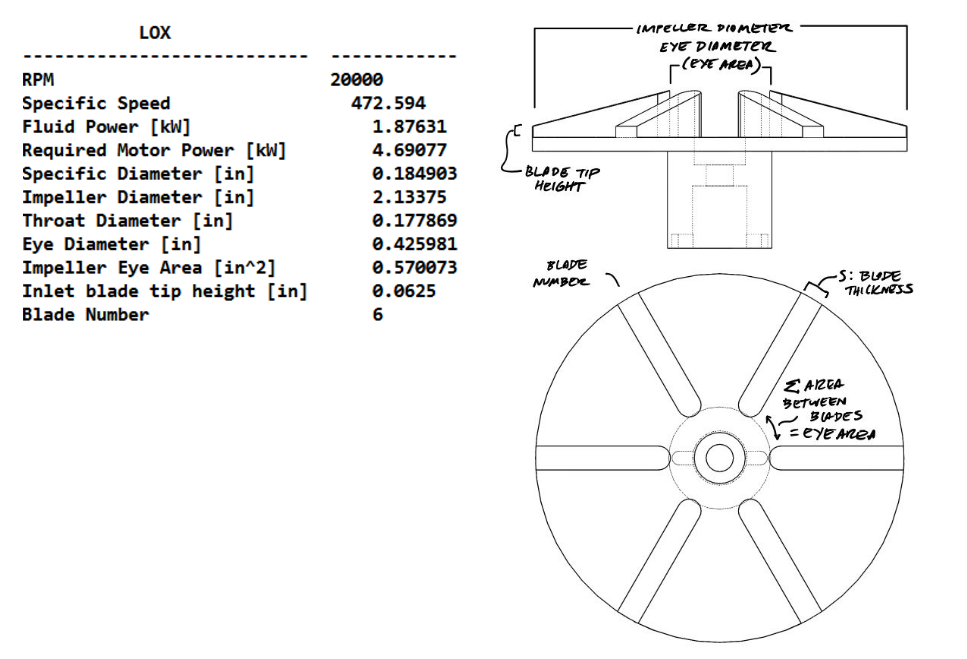
\includegraphics[width=\textwidth]{example_pump.png}
\caption{Example outputs from pump sizing python notebook and parameterized CAD impeller drawing output}
\end{figure}

\vspace{12pt}
\begin{figure}[!h]
\begin{centering}
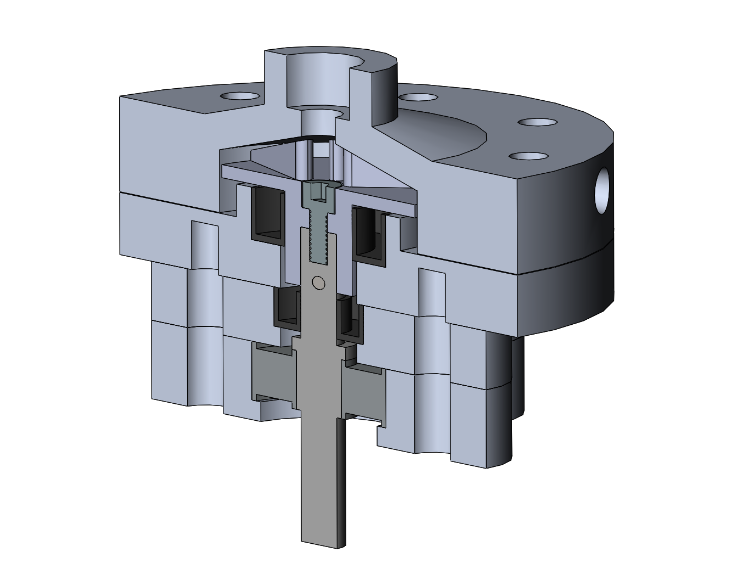
\includegraphics[width=0.5\textwidth]{Assem.png}
\caption{Example parameterized CAD pump assembly}
\end{centering}
\end{figure}
\newpage

\winsec{Subsystem decomposition: }{}
\vspace{12pt}
The EFS is comprised of four subsystems: the electric motor system , the controls and data acquisition system, the test stand, and the pump itself. \par
\vspace{12pt}
	The electric motor system is comprised of an electric motor, a battery, and an electronic speed controller (ESC). The data acquisition and controls system uses a Labview-Arduino interface to monitor the pump via pressure and temperature sensors and controls the system through solenoid valves and by directly controlling the motor’s speed controller. The test apparatus system is comprised of propellant and pressurant tanks and provides the propellant to the pump at a specified pressure. The pump itself is the center of the system, with the impeller being the core of the pump subsystem. The impeller may also be considered as a subsystem itself, as the requirements of the impeller dictate the requirements of the rest of the pump system components, including the housing, shaft, and bearings.\par
\vspace{12pt}
	
\begin{figure}[h]
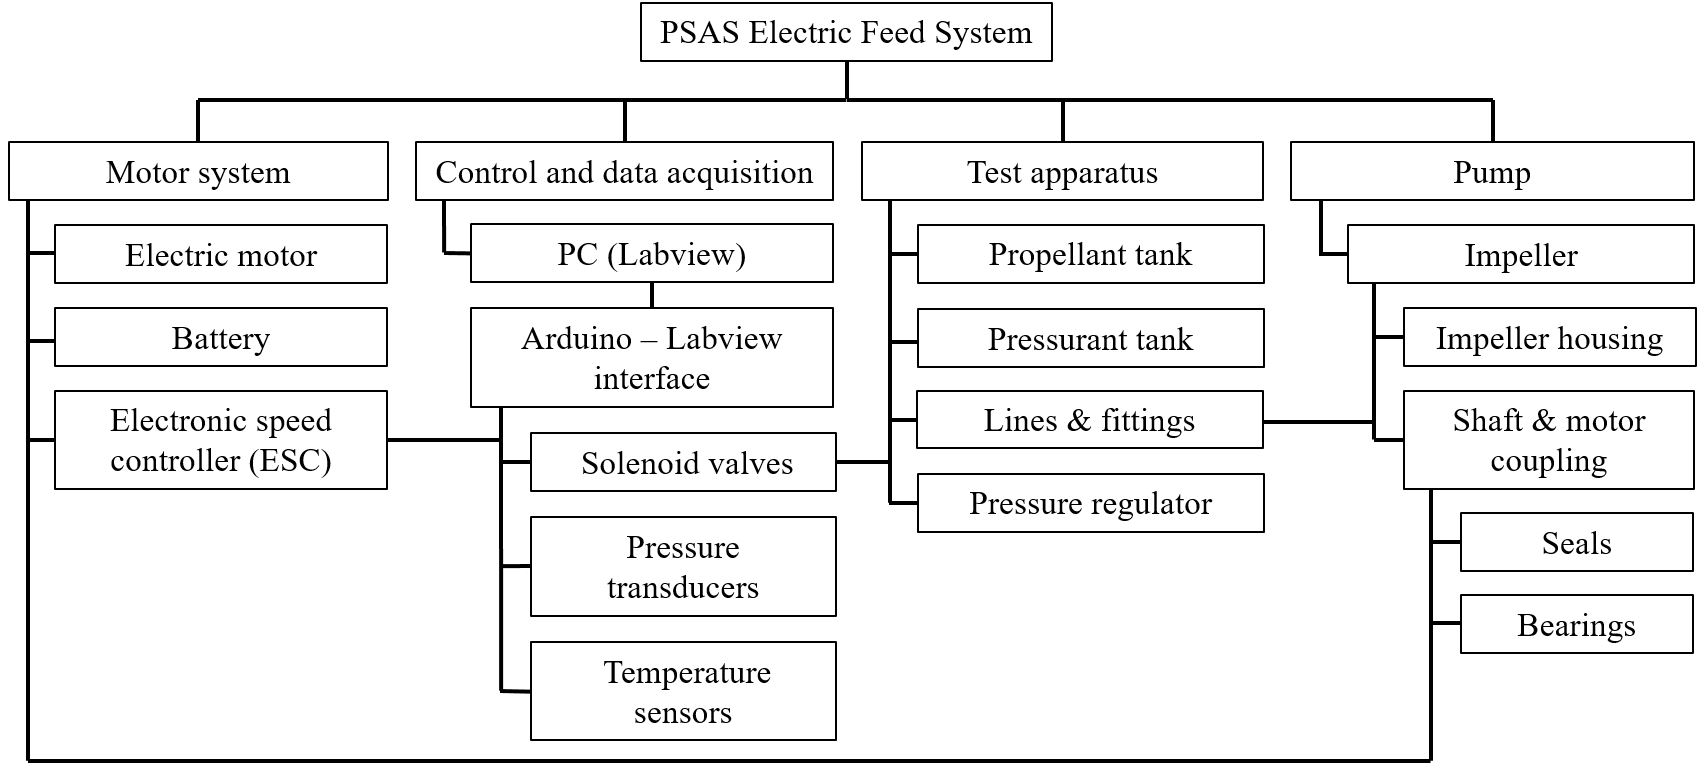
\includegraphics[width=\textwidth]{subsystem_decomposition_3_19_17.jpg}
\caption{Electric feed system hierarchical subsystem decomposition}
\end{figure}

	The motor system connects to the pump subsystem via a coupled shaft that joins the electric motor and the impeller, and the ESC is directly controlled by the Labview-Arduino interface of the controls system. The controls system bridges to the test apparatus by controlling the solenoid valves on the propellant and pressurant tanks, which feed the pump itself.\par

\begin{figure}[h]
\begin{center}
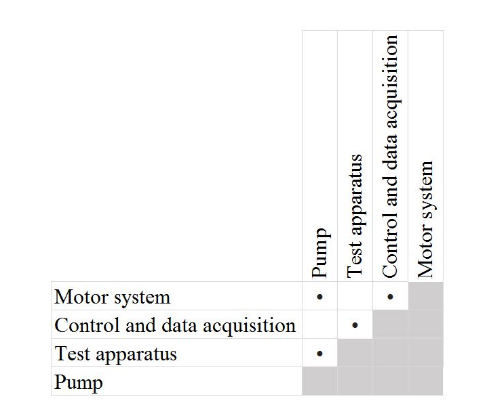
\includegraphics[width=0.45\textwidth]{Interface_matrix.png}
\caption{Subsystem interface matrix for the EFS}
\end{center}
\end{figure}

\winsec{Updates on Performance Measures: }{}
\winsub{Key system level performance measures}
The performance measures for the final prototype have remained constant as were provided in the project contract:\par


\begin{itemize}
\item The EFS pumps liquid isopropyl alcohol (IPA) at 1.3-1.4 lbm/s.
\item The EFS pumps liquid oxygen (LOX) at 1.6-1.8 lbm/s.
\item The EFS delivers a discharge pressure greater than 350 psi.
\item The EFS delivers a stable discharge pressure varying less than 10\%.
\item The EFS can sustain operational requirements for 20 seconds.
\item Prototype approximates a flight ready system in terms of mass (less than 10 kg).
\item The pump can be disassembled, moved, and assembled by 3 team members in under 1 hour. 
\end{itemize}

While these final prototype performance measures have not changed, the need for an independent set of requirements unique to the first prototype has become apparent. The first prototype’s intention is to provide feedback for the validation of our pump design theory and calculations, and until the project transitions to the development of the second prototype, the team is functioning under a temporary set of performance measurements unique to that objective:\par

\begin{itemize}
\item The first prototype achieves pressure, flow rate magnitude and stability within +/- 25\% of the final performance measure values. 
\item The first prototype includes a set of experimental impellers and housing variants sufficient to corroborate theory and optimize the second prototype design.
\item The first prototype can record inlet and outlet pressure, RPM and flow rate data at a resolution sufficient to allow accurate data analysis.
\item The first prototype can vary impeller RPM between 10,000 and 50,000 RPM
\item The first prototype can withstand discharge pressures up to 500 psi.
\item The first prototype can sustain operational requirements for 60 seconds.
\item The first prototype can be disassembled, moved, and assembled by 3 team members in under 1 hour. 
\item The first prototype impeller and impeller housing can be changed in under five minutes.
\item The first prototype pump water.
\end{itemize}

	These performance measurements represent the requirements of a test apparatus. The core pump performance metrics are not critical as long as they fall into a range that can be used to refine our pump design theory and calculations. If the first prototype could achieve > \textasciitilde250 psi, we could likely adapt our design to achieve the performance measurements required in the second prototype. Additional measurements unique to the first prototype test involve more rigorous data collection specifications, longer operational duration requirements, and a design accommodation for  easily interchangeable impellers and housings.\par
\vspace{12pt}
	Please note the 1st and 2nd prototype RM matrices for the pump subsystem included in the appendix. The goal of these competing matrices is to clarify that the first prototype has lax pump performance requirements but more stringent testing requirements. The second prototype’s priorities are more focused on the pump performance numbers.\par
\newpage

\winsub{Test plan for verifying performance}
\vspace{12pt}

\begin{table*}[!h]
\caption{Test platform control system}
\resizebox{\textwidth}{!}{%
\begin{tabular}{|c|cr|c|}
\hline
\textbf{Device: }&\textbf{Function: }&&\textbf{Control type: } \\ \hline \hline
Electric motor&&drive the propellant pumps&Electronic \\ \hline
Oxydizer main valve&& Open and close the main oxydizer line&Electronic \\ \hline
Fuel main valve&& Open and close the main fuel line& Electronic \\ \hline
Check valves&& Avoid pump overpressures&Automatic \\ \hline
Tank drain valves&& Evacuate the remaining propellants after burnout or in emergency shutoff&Electronic \\ \hline
Tank fill valves&&Fill tanks before testing& Manual \\ \hline
Pressurization valve&& Pressurizes propellant just before test start& Manual\\ \hline
\end{tabular}}
\end{table*}


\begin{table*}[!h]
\caption{Test performance measurement methods}
\resizebox{\textwidth}{!}{%
\begin{tabular}{|c|cr|cr|}
\hline
\textbf{Variable: }&\textbf{Monitoring device: }&&\textbf{Observations}&\\ \hline \hline
Combustion chamber pressure&&Pressure transducer&&Optionally an indirect method may be used \\ \hline
Injector head inlet pressure&&Pressure transducer&&Absolute pressure type with transducer \\ \hline
Propellants tank pressure&&Indirect measure&&Via gas tank pressure regulator working pressure \\ \hline
Pump rotational speed&&Tachometer&&coupled to motor shaft \\ \hline
Pump Torque&&Dynamometer&& Made using strain gauges\\ \hline
Required electrical power&&Indirect measure&&Sensing simultaneously motor current and voltage \\ \hline
Propellants flow rate&&Indirect measure&&Via pump flow characterization and motor speed sensing \\ \hline
\end{tabular}}
\end{table*}

\winsec{Planning Update: }{}
\vspace{12pt}
The EFS project is currently ahead of the milestone schedule anticipated in our 2/14/17 project plan, particularly for milestones involving the first water pumping prototype. First prototype testing was initially planned by 5/6/17 with data analysis completed by 5/22/17, but those milestones are currently expected to be completed three to four weeks early. This is unlikely to affect milestones involving the second, liquid oxygen pumping prototype, as the results of the first prototype test will determine whether additional design-test iteration of the first prototype will be needed to validate our theory and design before proceeding with the more challenging, liquid oxygen pumping second prototype. Being ahead of schedule is small relief given the daunting challenges of the final prototype’s requirements. Please see the updated Gantt chart in the appendix.\par



\newpage
\end{comment}

\pagenumbering{Roman}
\winsec{Appendix A1:}{ Updated Gantt Chart}
%---------------------------------%
%New Gantt Chart Goes here!%
%---------------------------------%

\begin{center}
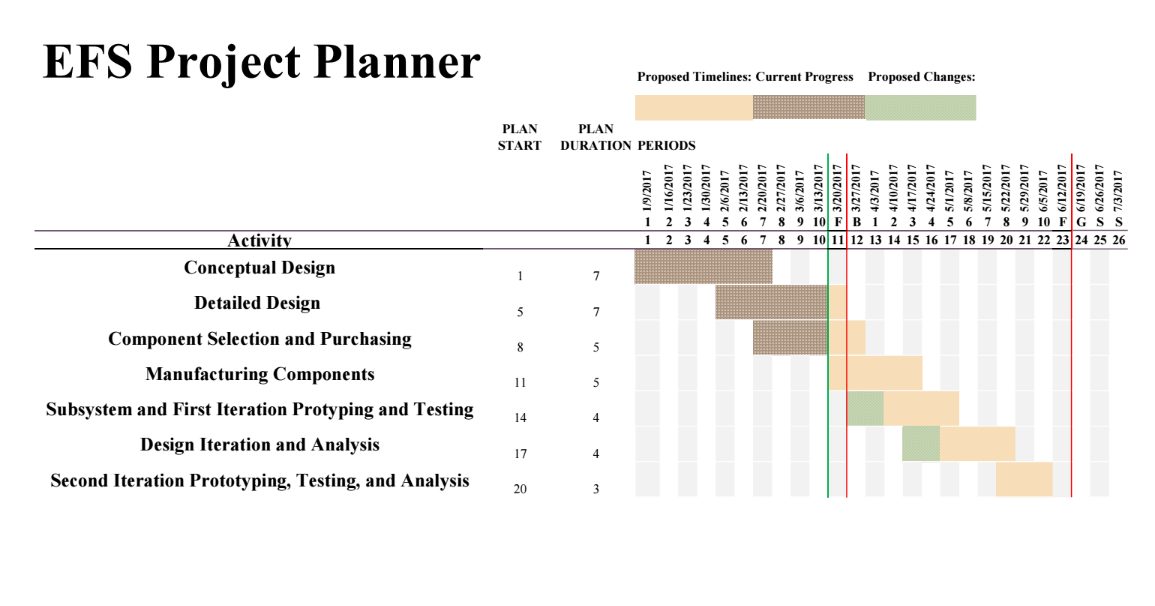
\includegraphics[width=1.3\textwidth,angle=270]{Gantt_chart.png}
\end{center}



\newpage
\winsec{Appendix A2:}{ Requirements and Measurements Matrix}
%---------------------------------%
% New RM matrix Goes here! %
%---------------------------------%

\setcounter{figure}{0} \renewcommand{\thefigure}{A.\arabic{figure}}

\begin{figure}[!h]
\begin{center}
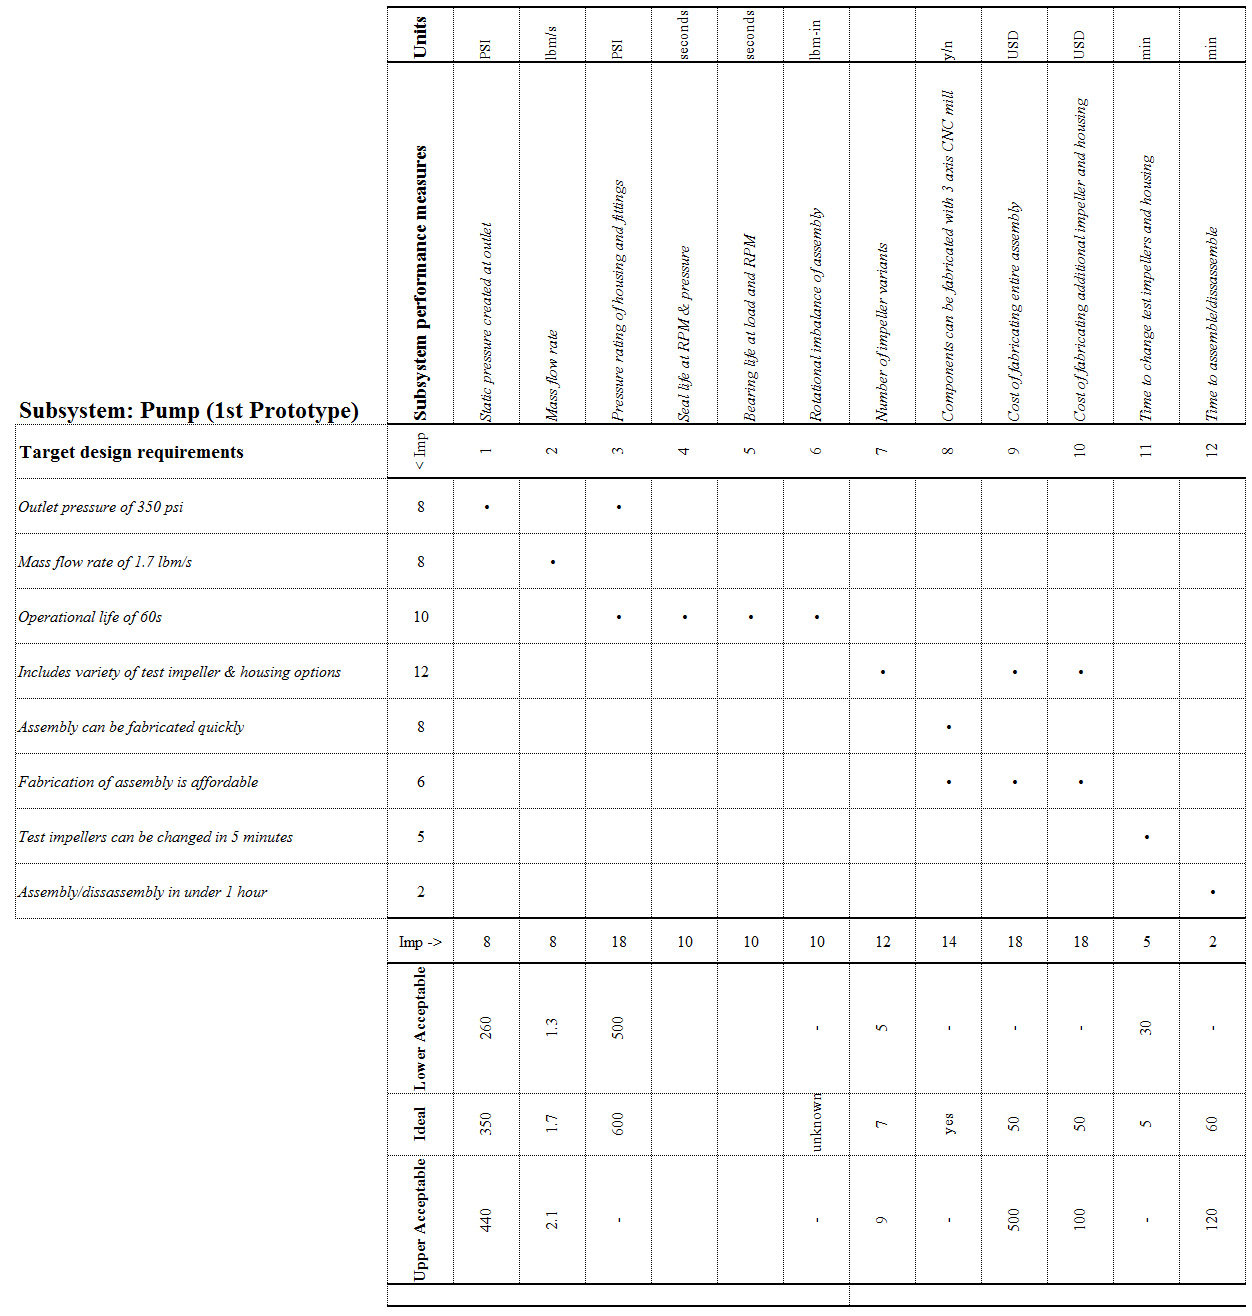
\includegraphics[width=\textwidth]{1st_prototype_RM_matrix.jpg}
\caption{Requirements/measurements matrix for the first prototype EFS}
\end{center}
\end{figure}
\newpage
\begin{figure}[!h]
\begin{center}
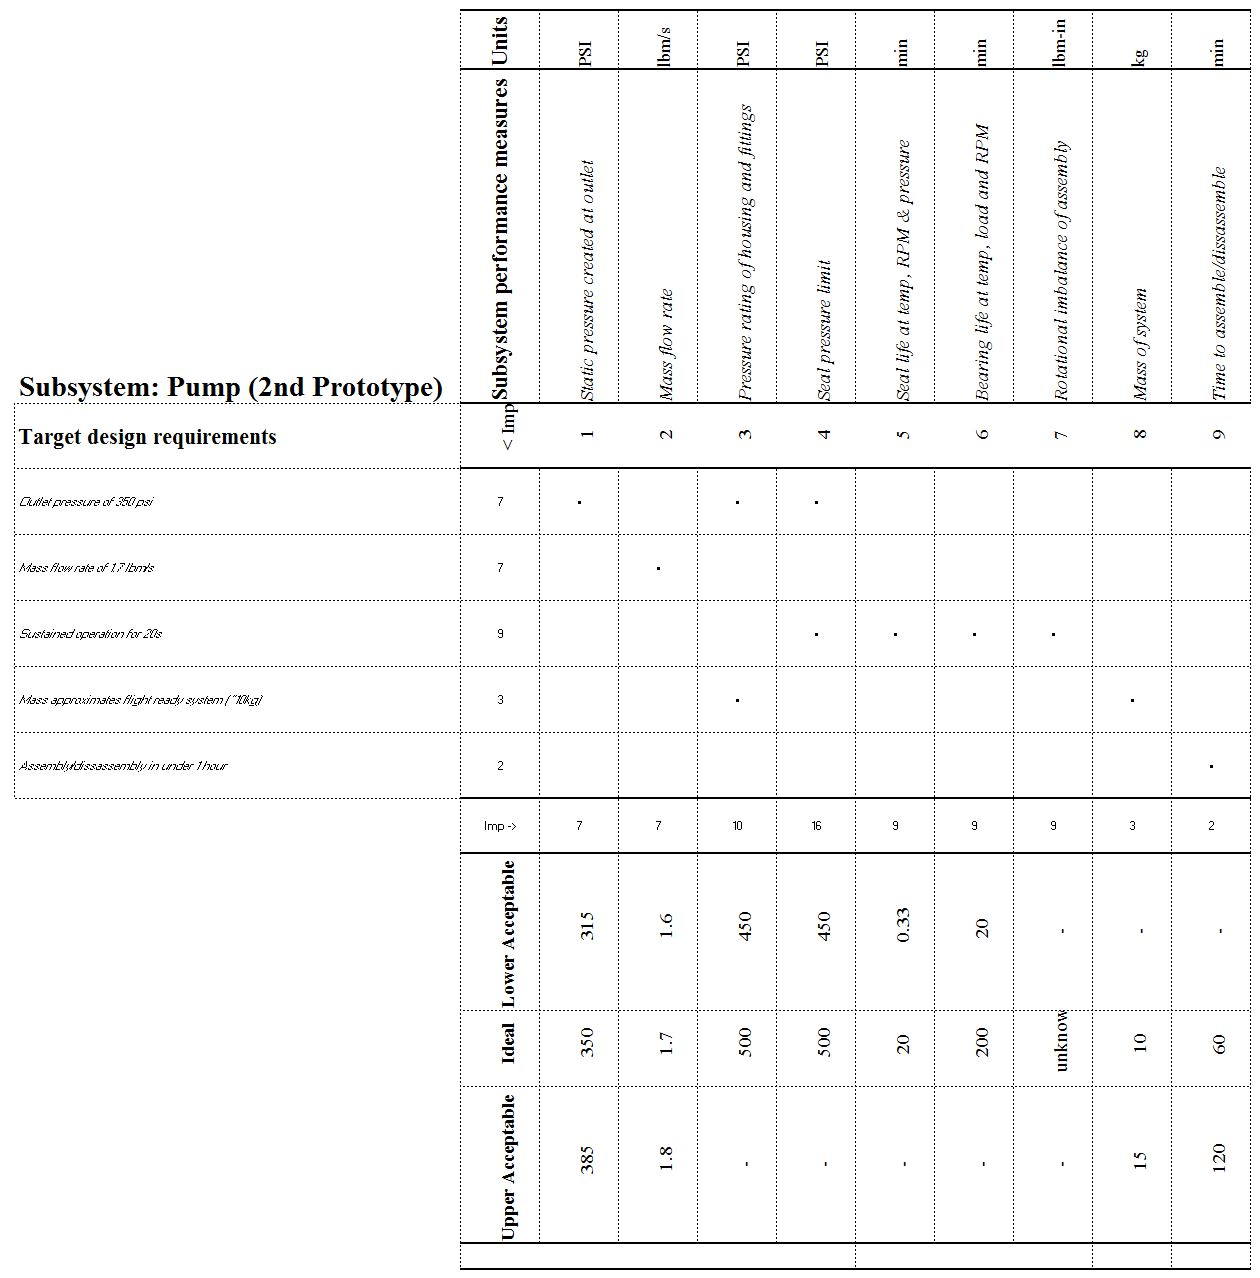
\includegraphics[width=\textwidth]{2nd_prototype_RM_matrix.jpg}
\caption{Requirements/measurements matrix for the second prototype EFS}
\end{center}
\end{figure}



\begin{comment}
\winsec{Appendix A3:}{ Bill of Materials}
%---------------------------------%
%     New BOM Goes here!     %
%---------------------------------%
\resizebox{\textwidth}{!}{%
\rowcolors{2}{gray!25}{white}
\begin{tabular}{|llcc|}
 \hline
\textbf{Part:}&\textbf{Description:}&\textbf{QTY:}&\textbf{Price:}\\ \hline
\textbf{Motor System:}&&&\\
Motor&Aquastar T20 3T&1&\$97.89\\
Speed controller&AquaStar 240A Water Cooled ESC&1&\$247.07\\
\textbf{Pump: }&&&\\
Aluminum stock&T4048 Aluminum&1&\$31.50\\
\textbf{Control and Data: }&&&\\
Arduino&Arduino Uno&1&\$0.00\\
Solenoid valves&&2&\\
Pressure Transducers (500 psi)&Ashcroft / Grainger G17M0215F2500&2&\$188.75\\
Pressure Gauge (600 psi)&Winters / Amazon PFP663ZRR1&2&\$19.44\\
Pressure Transducer (3000 psi)&Ashcroft / Grainger G17M0215F23000&1&\$188.75\\
Temperature sensors&&5&\\
\textbf{Test Apparatus: }&&&\\
Nitrogen Tank&LuxferL45J&2&\$0.00\\
7/8" to 1/2" compression fitting&Swagelok SS-810-1-10ST&2&\$20.80\\
1/2" to 1/4" tube adapter&Swagelok SS-400-R-8&2&\$11.18\\
1/4" Branch Tee&Swagelok SS-400-3-4TTM&1&\$28.88\\
Needle Valve&Dixon / Amazon MFS102&1&\$60.98\\
Flexible Tubing\&Associated Hose &4R2AT-4-204-B/E&1&\$32.70\\
Pipe Nitrogen&Swagelok SS-T4-S-035-20&12&\$2.57\\
Ferrule Male Connectors&Swagelok SS-400-1-4&5&\$7.35\\
1/4" Ferrule Tee&Swagelok SS-400-3&2&\$23.40\\
1/4" NPT Hex Nipple&Swagelok SS-4-HN&4&\$6.32\\
1/4" NPT/ 1/4" Ferrule Elbow&Swagelok SS-400-2-4&2&\$14.08\\
1/4" Female Tube Adapter&Swagelok SS-4-TA-7-4&4&\$10.15\\
1/2" Female Tube Adapter&Swagelok SS-4-TA-7-8&2&\$13.77\\
1/4" NPT Male Tube Adapter&Swagelok SS-4-TA-1-4&7&\$6.32\\
1/4" Ferrule Cross&Swagelok SS-400-4&1&\$42.54\\
Ethanol Regulator&Swagelok KCY1JRA412A20000&1&\$523.86\\
Oxygen Regulator&Swagelok KCY1JRA412A20000&1&\$523.86\\
Check Valves&Swagelok SS-4C4-1&2&\$48.55\\
Solenoids (Nitrogen)&Asco 8262H080&2&\$98.10\\
Manifold material&Alaskan Copper \& Brass 132132-3P&1&\$62.00\\
Relief Valves&Swagelok SS-4R3A5-SETB&2&\$151.49\\
Vent Valves&Asco 8262H214&2&\$131.08\\
Slic-Tite PTFE Thread Tape&La-Co/Amazon 44094&1&\$2.56\\
1/4" NPT Cross&Parker / Grainger 1/4 KMMOO-SS&1&\$74.55\\
\textbf{Misc: }&&&\\
Wire&Turnigy High Quality 8AWG Silicone Wire&2&\$7.00\\
Bullet connectors&Turnigy 8MM gold connectors&1&\$18.00\\
 \hline
\end{tabular}}
\end{comment}


\newpage

\end{document}